\documentclass[utf8]{beamer}
\usepackage{listings}
\usepackage[russian]{babel}
\usepackage{verbatim}
\usepackage{color}
\usetheme{Malmoe}
\title{LTE Radio Access Network}
\author {Компьютерные сети и протоколы}
\date{Лекция 9}
\begin{document}
%--------------------------------------------------------------------------------
\begin{frame}
\titlepage
\end{frame}
%--------------------------------------------------------------------------------
\begin{frame}
\frametitle{Что такое LTE?}
Разработка LTE началась в 2004 году\ldots
\begin{itemize}
\item Принципиально новый радио-интерфейс для \emph{пакетной} сети передачи данных
	\begin{itemize}
	 \item Увеличение пиковой пропускной способности сети
	 \item Высокая спектральная эффективность (бит/Гц/с)
	\end{itemize}
\item Гибкость в управлении спектром
\item Разработка улучшенной архитектуры сети (SAE) -- радиодоступа (E-UTRAN) и ядра сети (EPC -- Evolved Packet Core)
\end{itemize}
\end{frame}
%--------------------------------------------------------------------------------
\begin{frame}
\frametitle{Схема передачи в LTE RAN}
\begin{itemize}
 \item[8] Использование OFDMA в Downlink,  DFT-spread OFDM в Uplink + гибкое управление спектром
 \item[8] Использование FDD и TDD
 \item[8] Использование MIMO (до 8 антенн)
 \item[8] Использование \emph{одного} набора частот всеми базовыми станциями (eNodeB) и координация интерференции
 \item[8] Использование информации о канале передачи при планировании доступа к среде
 \item[8] Улучшенные методы кодирования, исправления ошибок передачи (Hybrid ARQ)
 \item[9] Синхронная широковещательная передача
 \item[10] Использование CoMP, Relaying и агрегации полос частот
\end{itemize}
\begin{center}
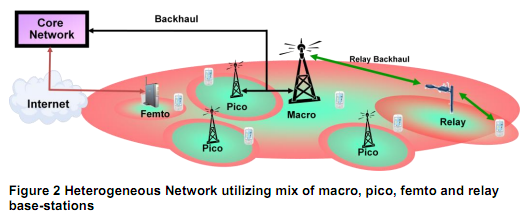
\includegraphics[width=0.5\textwidth]{pic/relay.png}
\end{center}
\end{frame}
%--------------------------------------------------------------------------------
\begin{frame}
\frametitle{Почему широкополосные системы связи?}
$$
R = BW\cdot\log_2\Big(1 + \frac{S}{N}\Big)
$$
Введем энергию, принимаемую на один бит:  $E_b=\frac{S}{R}$ и шум на один Герц $N_0 = \frac{N}{BW}$. Тогда:
$$
R\leq C=BW\cdot\log_2\Big(1 + \frac{S}{N}\Big)=BW\cdot\log_2\Big(1+ \frac{E_B\cdot R}{N_0 \cdot BW}\Big)
$$
$$
\gamma = \frac{R}{BW}\Big[\frac{\textrm{бит/c}}{\textrm{Гц}}\Big] \Rightarrow \gamma \leq\log_2\Big(1+\gamma\cdot\frac{E_b}{N_0}\Big) \Rightarrow \frac{E_b}{N_0} \geq \frac{2^{\gamma}-1}{\gamma}
$$
\begin{center}
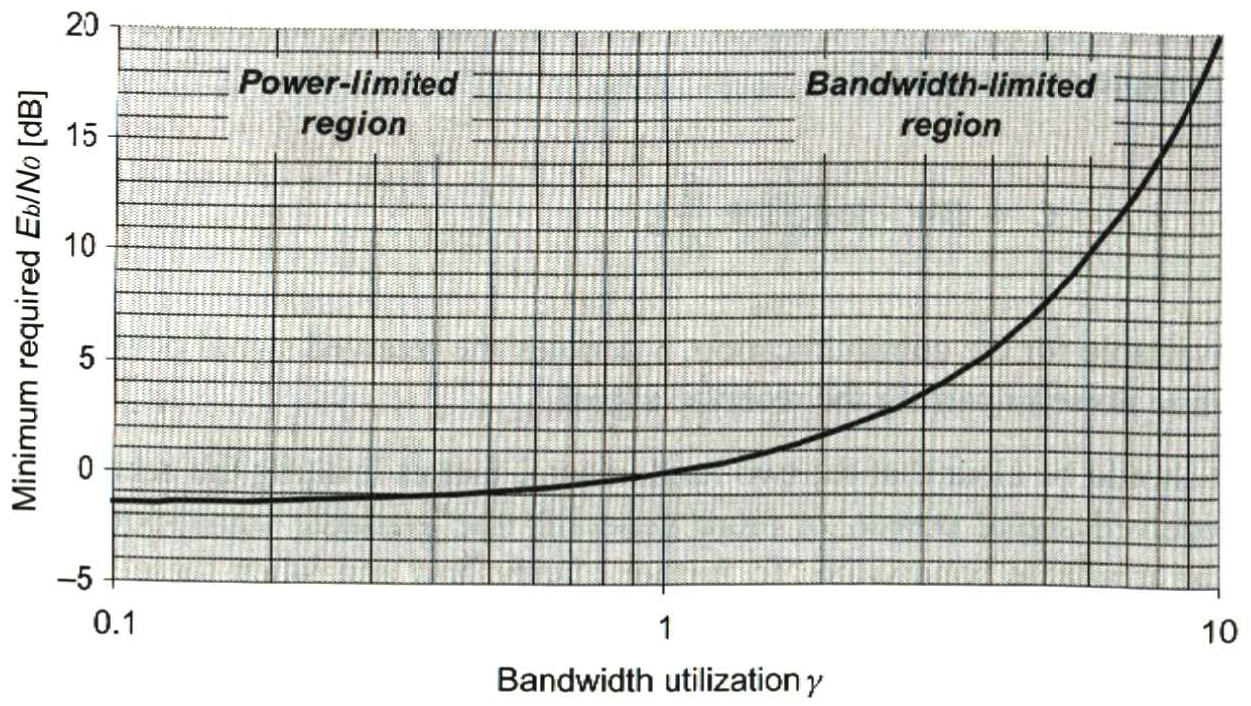
\includegraphics[width=0.5\textwidth]{pic/shannon.png}
\end{center}
\end{frame}
%--------------------------------------------------------------------------------
\begin{frame}
\frametitle{Почему OFDM?}
\begin{center}
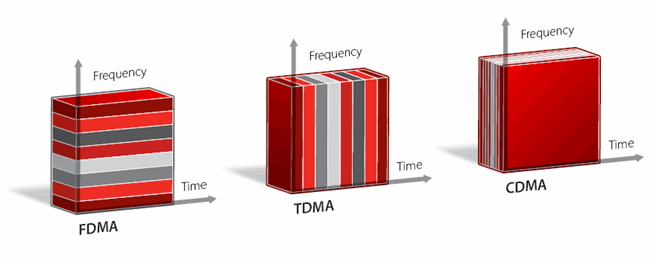
\includegraphics[width=0.5\textwidth]{pic/fdm-tdm-cdm.png}
\end{center}
\begin{description}
\item[FDMA] удобство организации Uplink. Один терминал не получит всю пропускную способность
\item[TDMA] высока вероятность пустых временных слотов и низкая энергоэффективность при небольших скоростях передачи
\item[CDMA] технически сложно реализуем из-за интерференции между абонентами (хотя теоретически выигрышнее)
\end{description}
\begin{block}{OFDMA}
Эффективное ``двумерное'' использование ресурса как по времени, так и по частоте
\end{block}
\end{frame}
%--------------------------------------------------------------------------------
\begin{frame}
\frametitle{Единицы измерения в LTE}
\begin{description}
\item[Resource Block] -- 12 поднесущих $\times$ 7 слотов (Urban!)
\item[SubFrame] -- 2 слота  $\times$ 7 2 поднесущих
\end{description}
\begin{center}
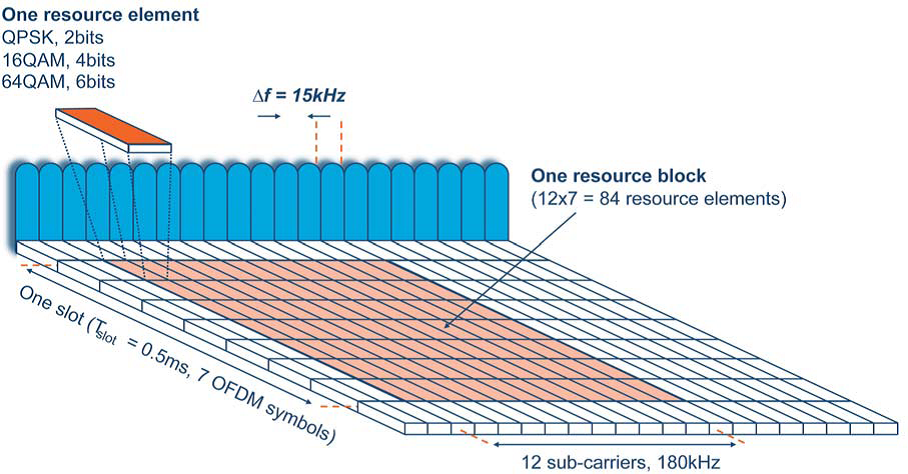
\includegraphics[width=\textwidth]{pic/rb-re.png}
\end{center}
\end{frame}
%--------------------------------------------------------------------------------
\begin{frame}
\frametitle{Временная структура кадра}
\centering
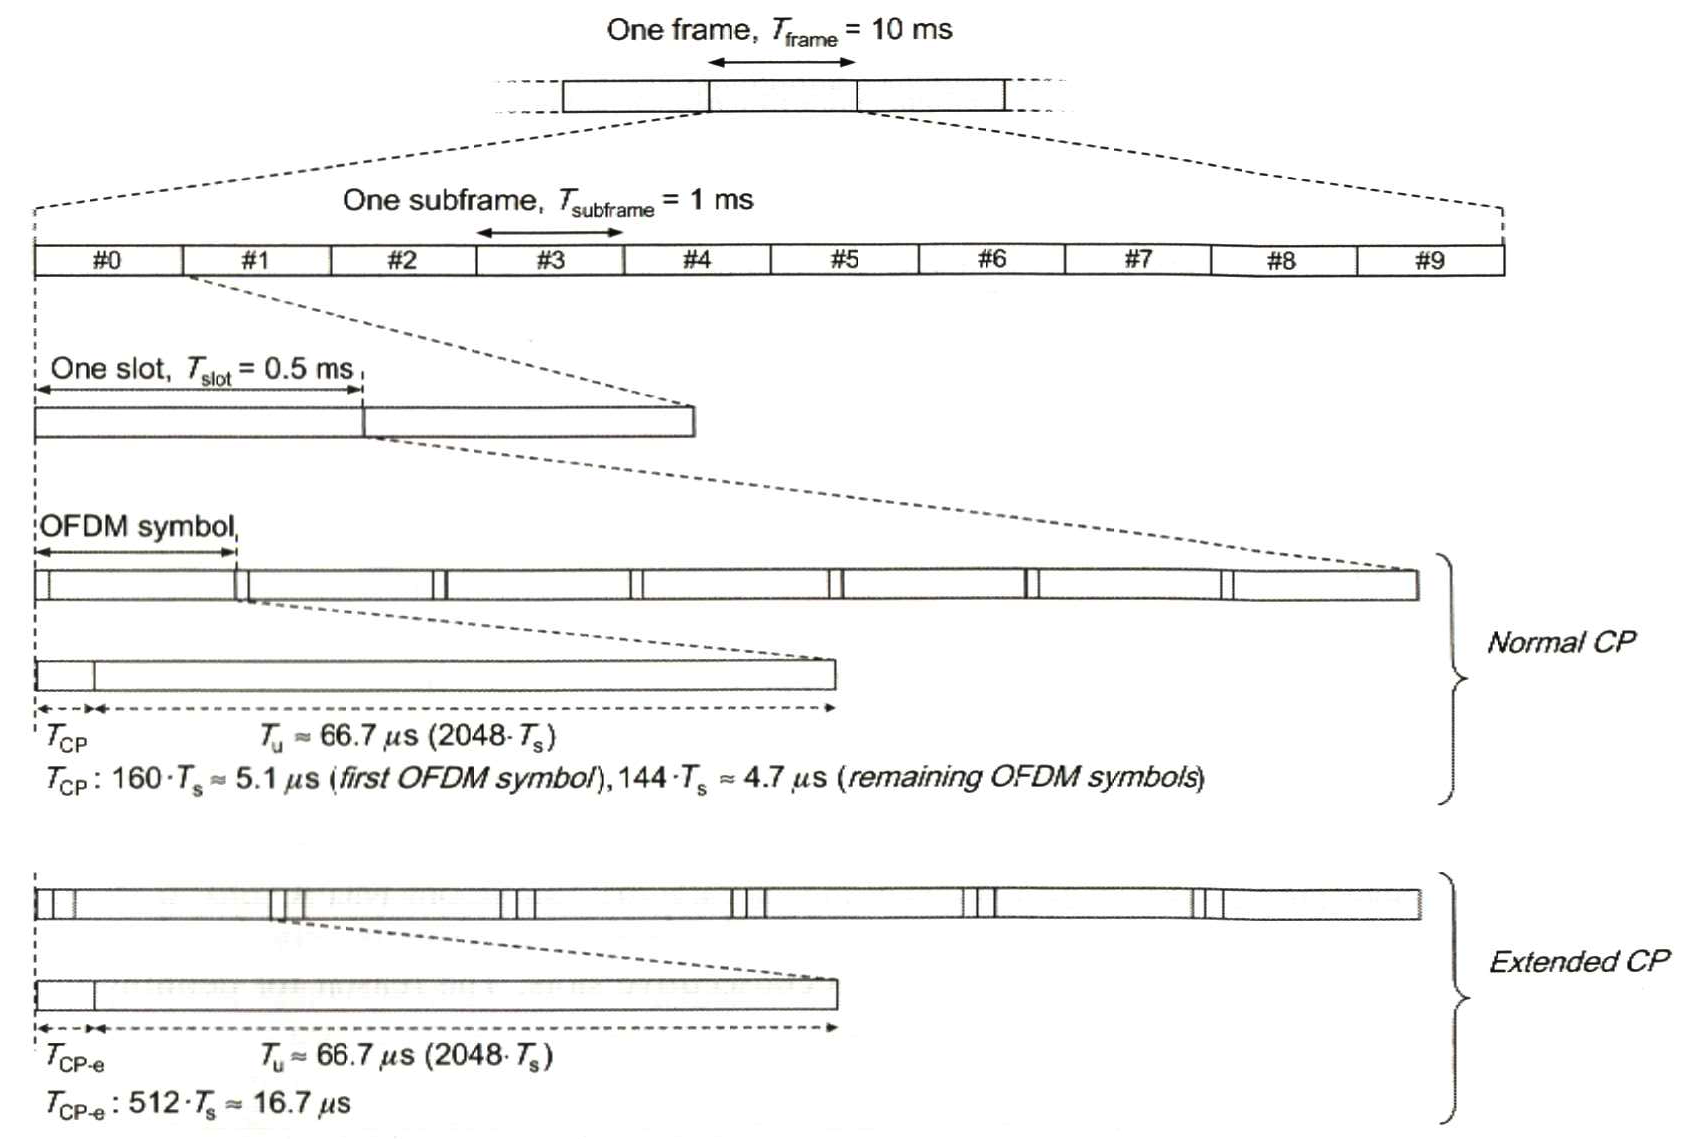
\includegraphics[width=\textwidth]{pic/time-domain.png}
\end{frame}
%--------------------------------------------------------------------------------
\begin{frame}
\frametitle{Эффективное планирование передач}
\centering
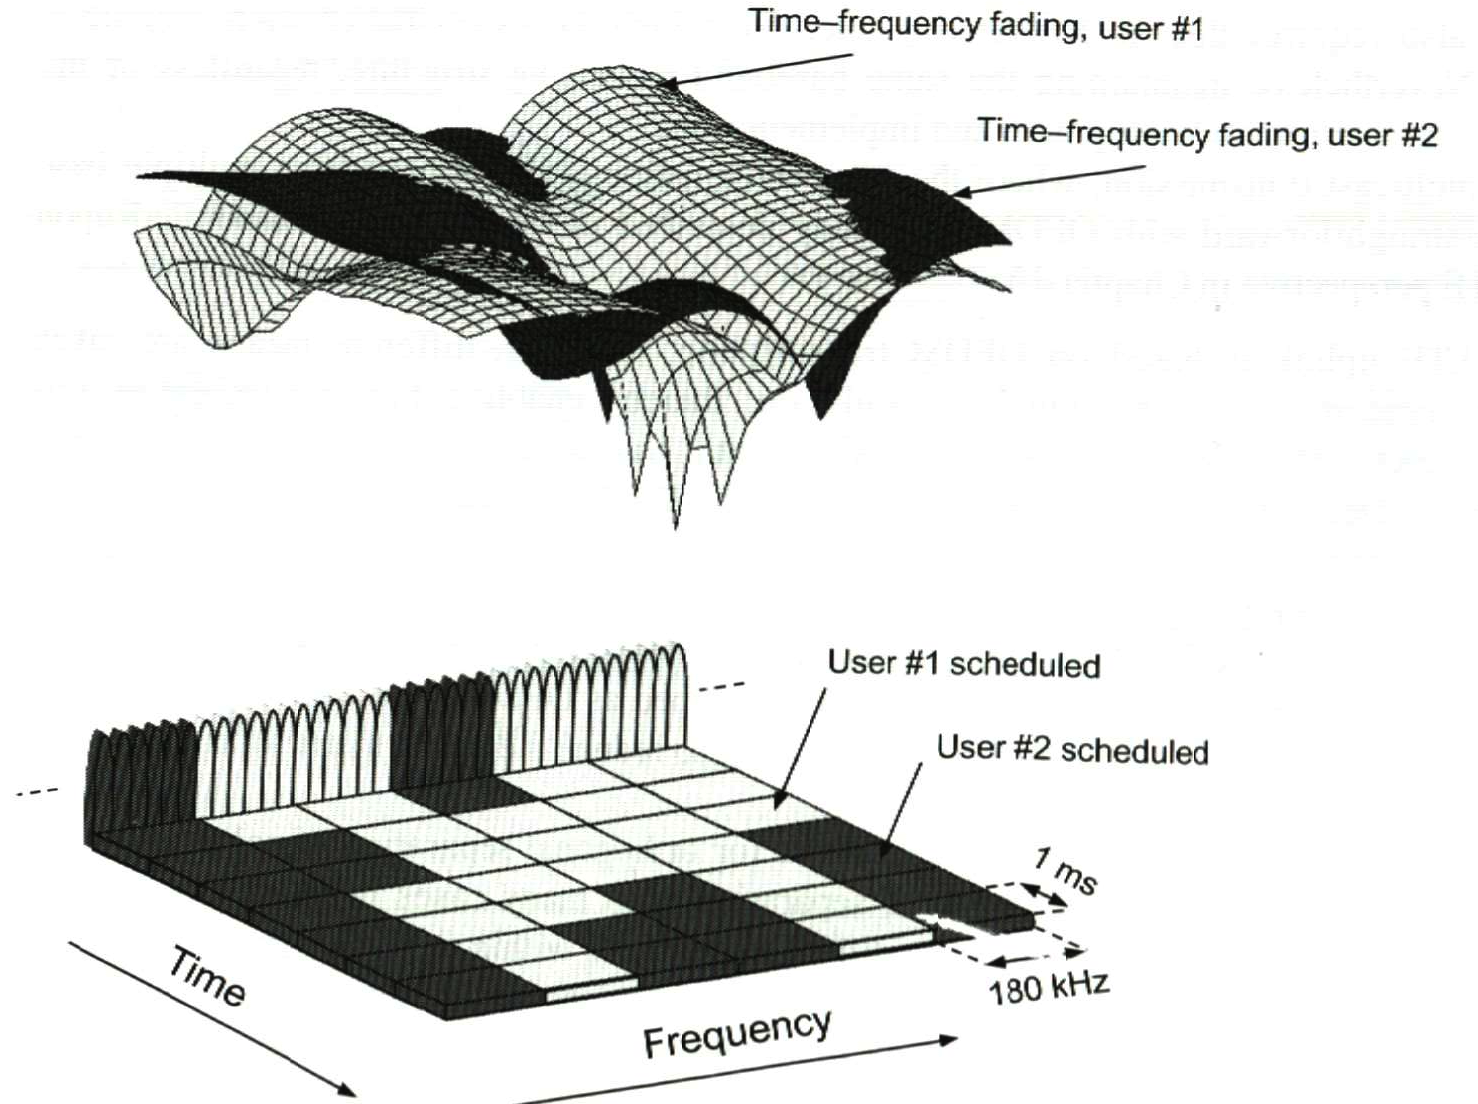
\includegraphics[width=\textwidth]{pic/scheduling.png}
\end{frame}
%--------------------------------------------------------------------------------
%--------------------------------------------------------------------------------
\begin{frame}
\frametitle{Что такое DFT-spread OFDM?}
\begin{itemize}
\item Как выделить ровно столько спектра, сколько нужно?
\item Как не ``залезть'' вне выделенной полосы?
\item Как снизить Peak-to-Average-Ratio (то есть удешевить мобильные телефоны)
\end{itemize}
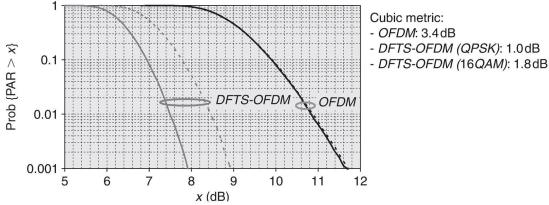
\includegraphics[width=0.5\textwidth]{pic/par-for-ofdm-and-ds-fdma.jpg}
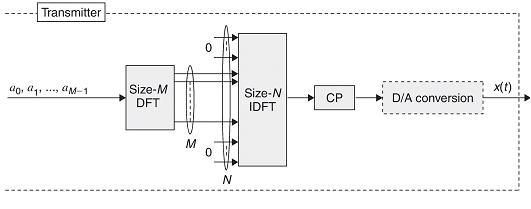
\includegraphics[width=0.5\textwidth]{pic/dts-fdma.jpg}
\end{frame}
%--------------------------------------------------------------------------------
\begin{frame}
\frametitle{Частотное разнесение}
\begin{center}
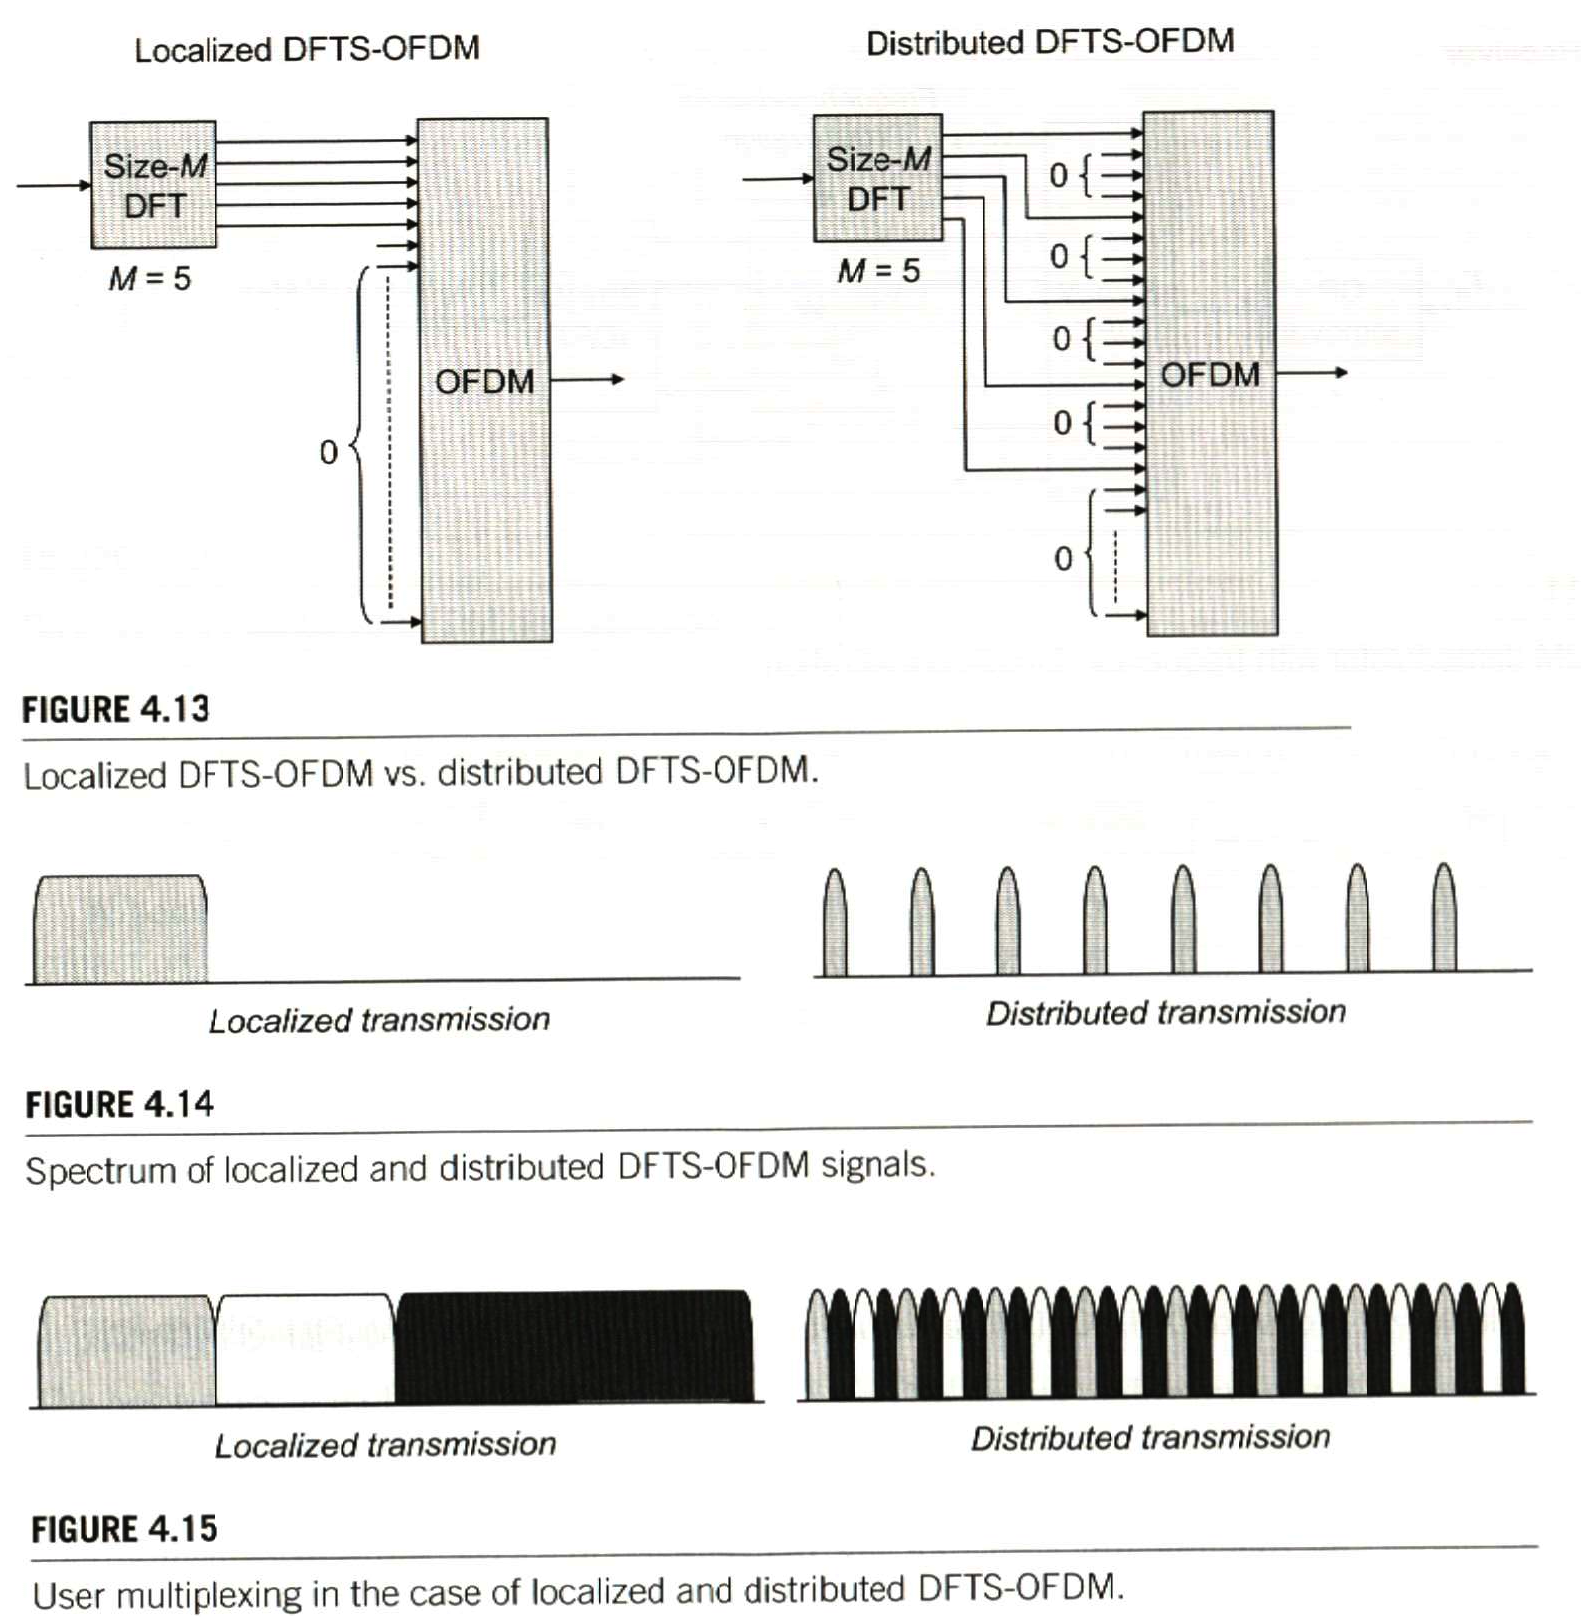
\includegraphics[width=0.75\textwidth]{pic/sc-fdma-distributed.png}
\end{center}
\end{frame}
%--------------------------------------------------------------------------------
\begin{frame}
\frametitle{Зачем отбрасывать пакеты с ошибками? Chase Combining}
\begin{center}
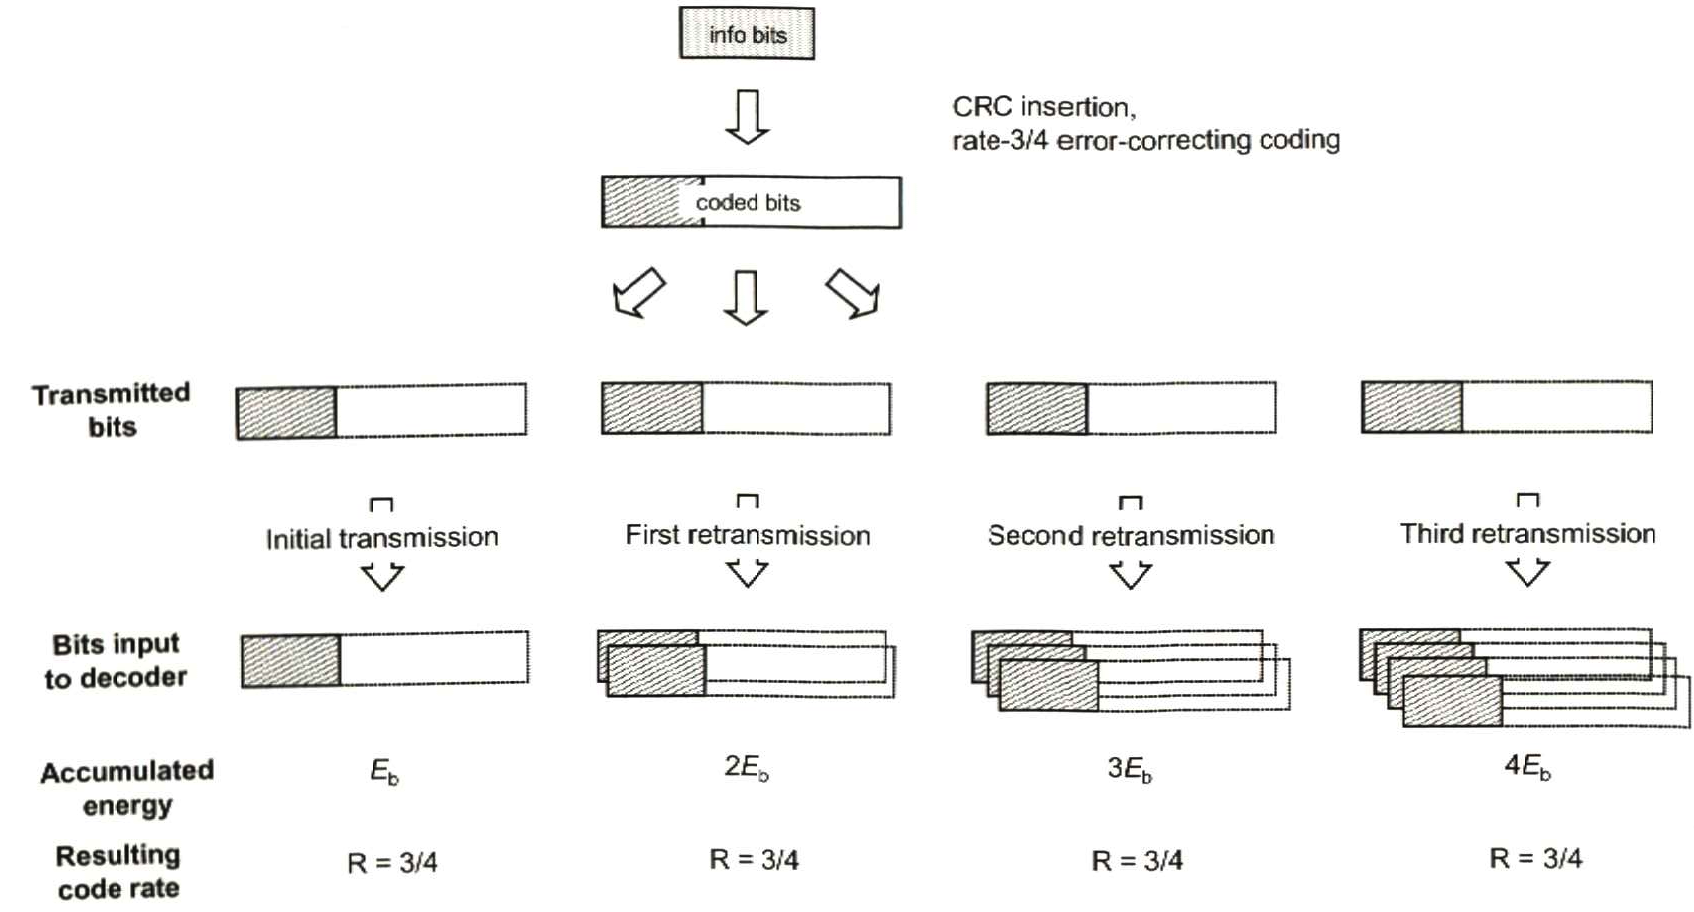
\includegraphics[width=\textwidth]{pic/chase-combining.png}
\end{center}
\end{frame}
%--------------------------------------------------------------------------------
\begin{frame}
\frametitle{Chase Combining + Modulation Scheme? Incremental Redundancy!}
\begin{center}
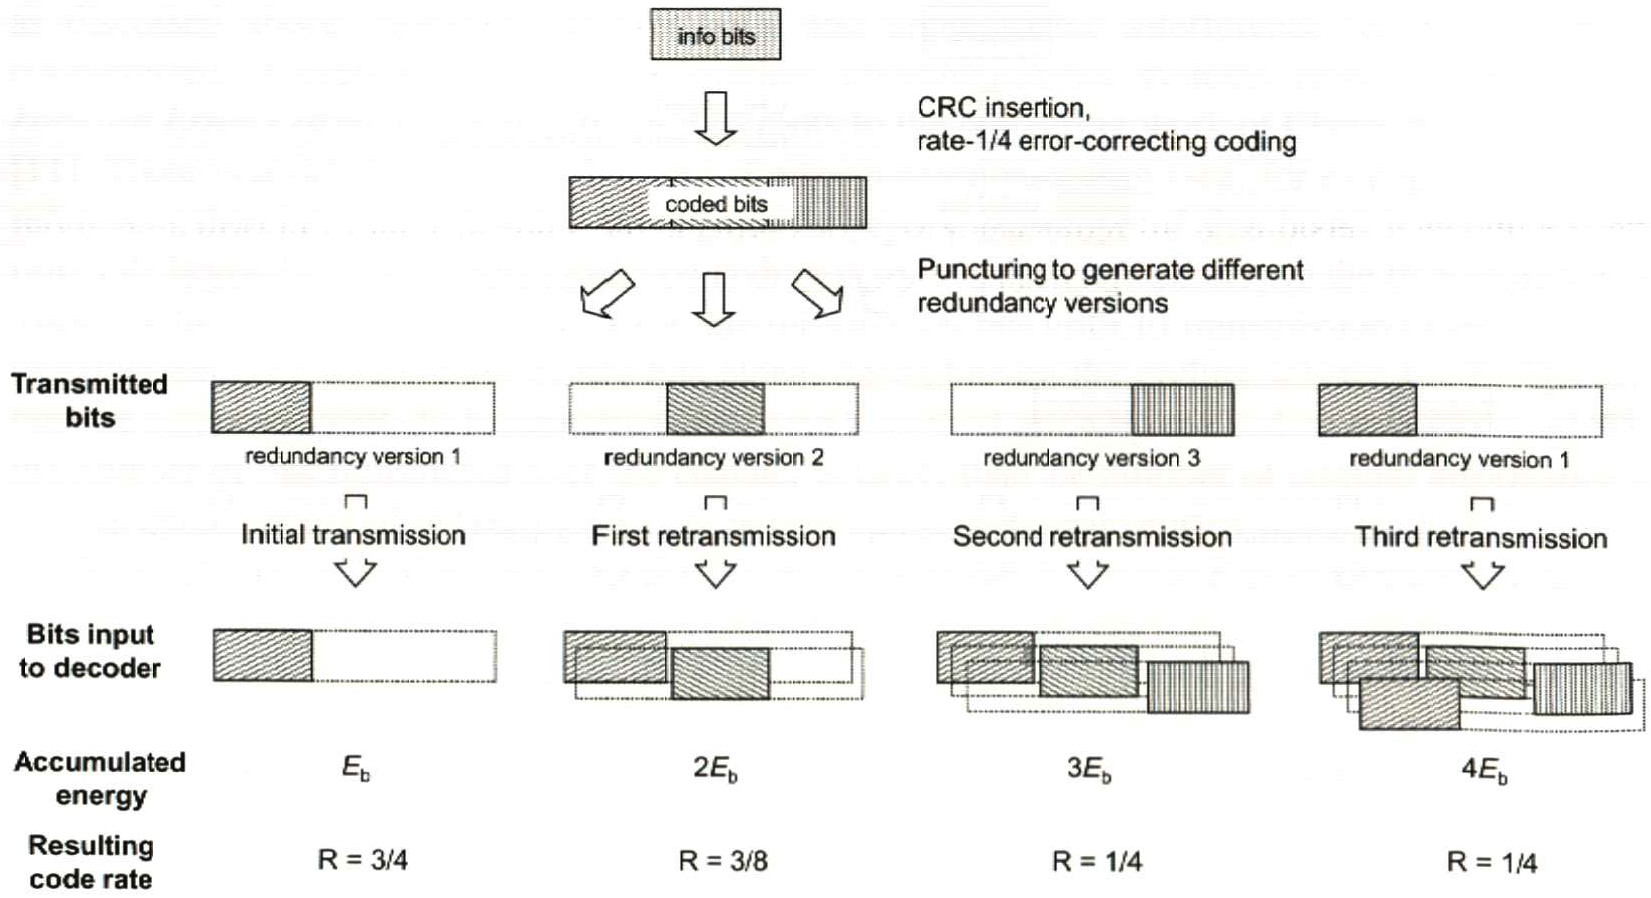
\includegraphics[width=\textwidth]{pic/incremental-redundancy.png}
\end{center}
\end{frame}
%--------------------------------------------------------------------------------
\begin{frame}
\frametitle{Архитектура сети LTE-RAN}
\begin{center}
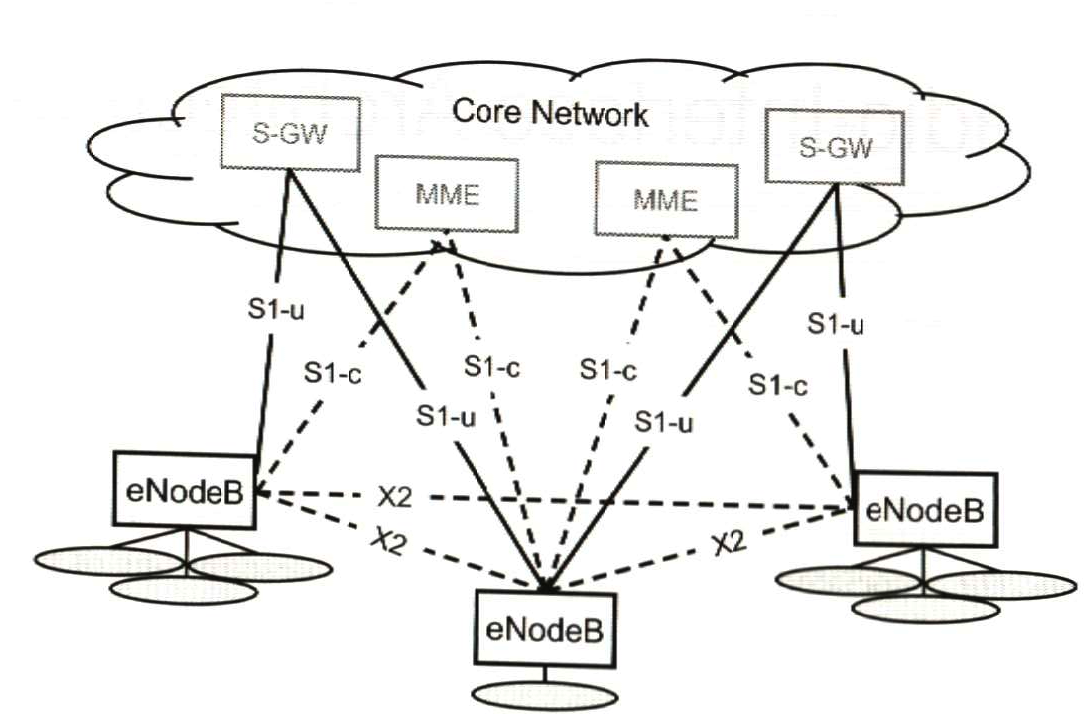
\includegraphics[width=\textwidth]{pic/ran-ifaces.png}
\end{center}
\end{frame}
%--------------------------------------------------------------------------------
%%--------------------------------------------------------------------------------
\begin{frame}
\frametitle{Структура Downlink каналов}
\begin{center}
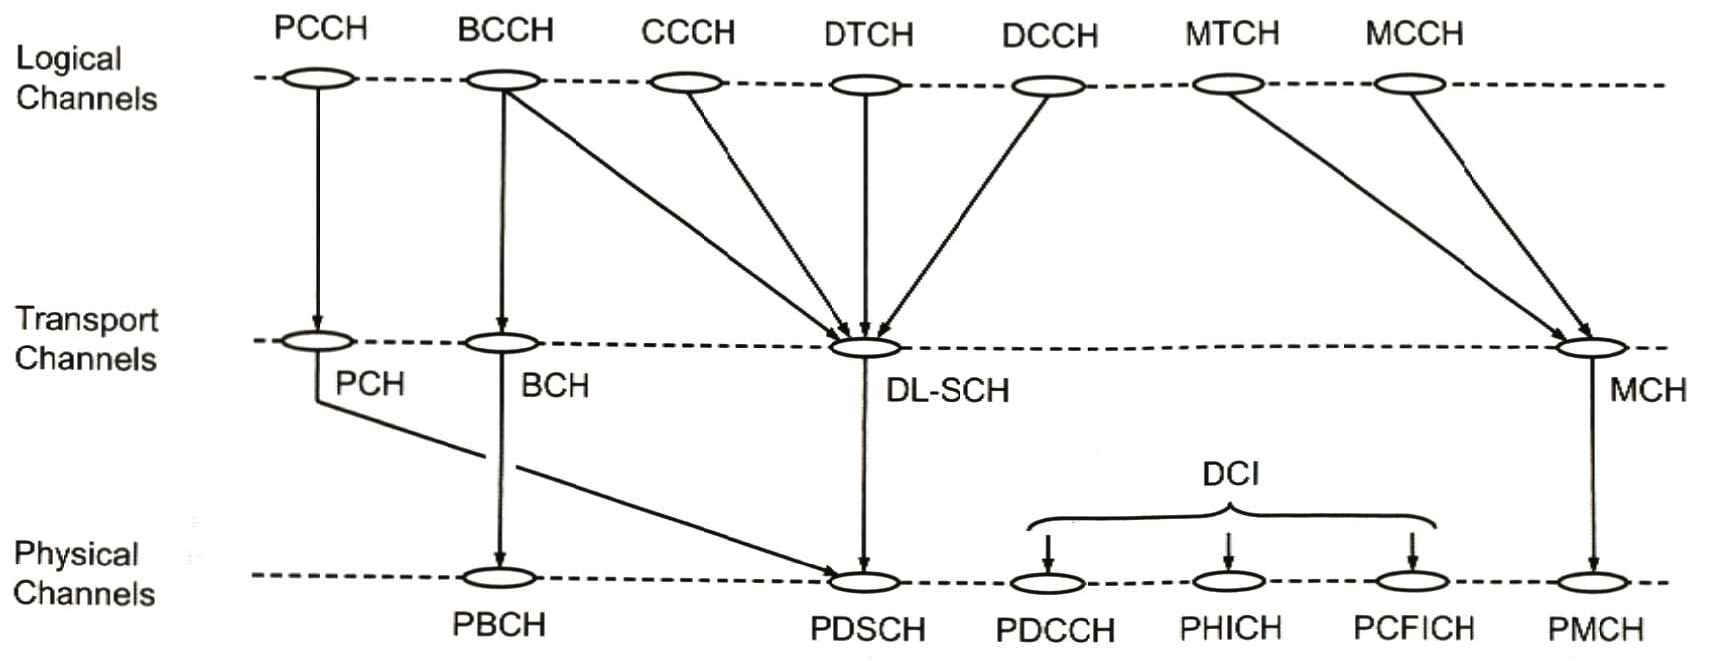
\includegraphics[width=\textwidth]{pic/DL-channels.png}
\end{center}
\end{frame}
\end {document}
